\documentclass[main.tex]{subfiles}
\begin{document}

\section{Learner's Tool}
\setcounter{section}{8}
%\setcounter{table}{0}
%\setcounter{figure}{0}

The previous chapters describe several systems for classifying texts as native and nonnative based on grammatical features. The accuracy of these systems varies from approximately 70\% to 90\%. While such classifiers are interesting and may have some utility in and of themselves, it is worth exploring whether these can form the foundation of an educational tool for learners of English. An effort has been made, when examining the decision trees of the various classification systems, to find linguistic reasons behind the classifiers' choice of attributes. It has been found that some attributes are used in ways which are very easy to interpret, based on the grammars of English and Spanish and the concept of L1-transfer, while others seem incomprehensible. This linguistic analysis is important, as it gives clues as to which attributes might play a useful part in a learning tool and which should be excluded. This chapter seeks to further analyze the attributes used by the classifiers in light of their utility in a learner's tool and to sketch out a possible design for such a tool.

Much of the complexity of any piece of user-oriented software is in the interface, but that will not be discussed in detail here. Suffice it to say that the program would allow the user, a learner of English, to enter a selection of English text that he or she has written. Because this system would be based on the frequency of textual attributes, the text would need to be long enough for the system to measure these frequencies with some level of statistical significance. Having entered a text, the user would then be presented with the output. This output would inform the user that certain features identify the text as nonnative, or that the system could not distinguish it from native text. In the former case, the system would show the user which features of the text are responsible for this classification and, when possible, would display all passages of the text that exhibited these features.

Identifying these features could be easily done if the system is using decision trees, whether generated by the C4.5 algorithm or by a similar algorithm. Consider any of the decision trees shown in the previous chapters. When one of these trees labels a text as nonnative, it associates the text with a particular leaf on the tree. From the leaf to the root there is a unique path that passes through all of the decision nodes which were used in classifying the text. Each of these decision nodes considers a single attribute, and these attributes are those that most strongly mark the text as nonnative. It would not be difficult, using Weka, for instance, to implement a version of C4.5 that generates decision trees which output all attributes used in a particular classification, in addition to the class itself. The system could use a single tree, trained on all attributes, or it could use multiple trees. These trees might correspond to grammatically distinct attribute sets, as do the trees shown in the previous chapters, or they might be the various trees of a Random Forest classifier. Using multiple trees could enable the system to present the user with a wider range of features.

The passages which exhibit the telltale features could then be located using tables generated when the system initially identified the features. Many of these textual features would be examples of overuse of various grammatical constructions, and the user could focus on the displayed passages as he or she revises the text. Others, however, would be examples of underuse. In this case, the system would only be able to identify positive examples in the text, or perhaps no examples at all, and it would be up to the user to find the appropriate places in which to use the relevant construction. A more sophisticated system might group certain features together in complementary or nearly complementary pairs (e.g., modals and phrasal modals), and then use the complement of the underused feature to suggest areas for revision. The user could then edit the text and let the system reevaluate it. Eventually, if the user was able to make appropriate changes, there would be a change in how the text was classified. The system might still classify it as nonnative, but would do so at a different leaf node in the tree, with a different set of responsible attributes. The cycle of revision and reevaluation could continue until the system classifies the text as native. Figure~\ref{fig:mockup} shows an example of what the interface of such a program might look like.
\begin{figure}[htbp]
\centering
\fbox{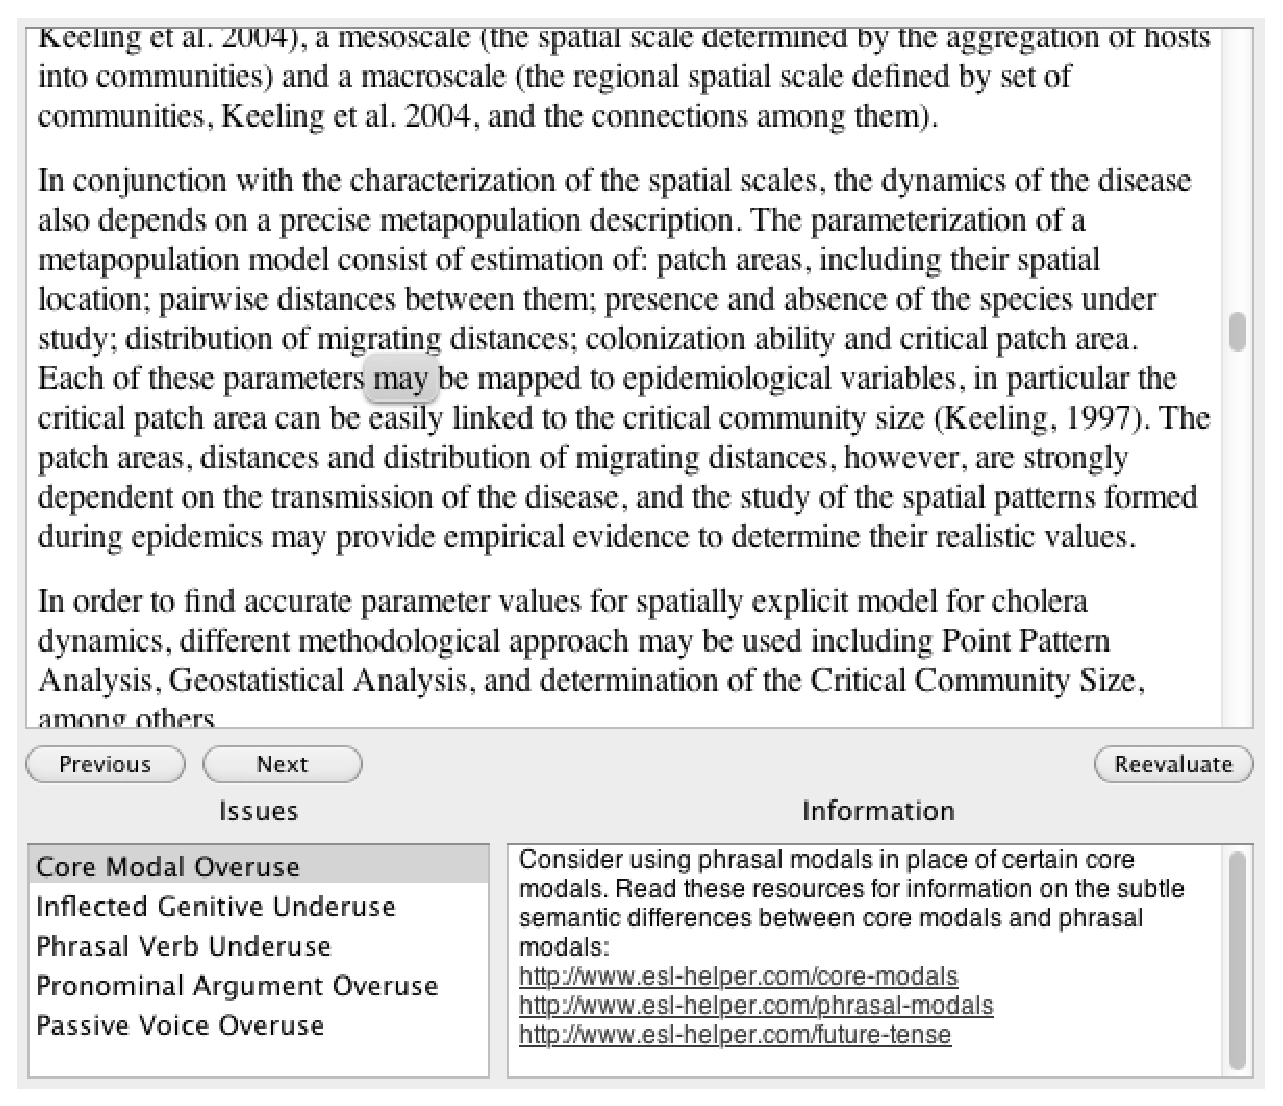
\includegraphics[scale=0.6]{tools-screenshot-bw.eps}}
\caption{Mock-up of the Interface of an ESL Learner's Tool}
\label{fig:mockup}
\end{figure}
In this mock-up, the large top pane contains the text entered by the user. The bottom left pane contains a list of issues (i.e., features) which identify the text as nonnative. Clicking on one of these issues causes the top pane to highlight the first instance of the issue. The user could then use the ``Next'' and ``Previous'' buttons to navigate through all such instances. At the same time, the bottom right pane shows general information on the topic and provides links to additional material.

An alternate system could be integrated with a word-processor and analyze the text dynamically as the user writes. In this case, the classification process would go on continuously in the background, only showing information regarding overuse and underuse when the text reaches a suitable length, and then providing feedback on each sentence as it is entered.
\begin{comment}
The interface could even include a ``nativeness meter,'' giving real-time feedback at a glance.
\end{comment}

\biblio
\end{document}